\documentclass [a4paper,11pt] {article}
%\pdfpagewidth\paperwidth
%\pdfpageheight\paperheight
\usepackage[utf8]{inputenc}
\usepackage[english]{babel}
\usepackage{natbib}
\usepackage{graphicx}
\usepackage{mathtools}
\usepackage[top=3cm,bottom=3cm,left=2.5cm,right=2.5cm,headsep=10pt,a4paper]{geometry} % Page margins
\usepackage{color}
\usepackage{amsmath, amsfonts, amsthm}
\usepackage[T1]{fontenc}
\usepackage[normalem]{ulem}
\usepackage[bottom]{footmisc}
\usepackage{hyperref}
\usepackage{epsfig}
\usepackage{plain}
\usepackage{listings}
\usepackage{titlesec} % per formato custom dei titoli dei capitoli
\usepackage{caption}
\usepackage{multirow}
\usepackage{array}
\usepackage{hyperref}
\setcounter{secnumdepth}{5}
\usepackage[cache=false]{minted} %outputdir needed to work with texpad , outputdir=.texpadtmp
\usepackage{pgfplots}
\usepackage{pgfmath}
\usepackage{subcaption}
\usepackage[official]{eurosym}
\usepackage{bm}
\usepackage[makeroom]{cancel}

\usepackage{diagbox}

\usepackage{colortbl, xcolor} %Colored celles in tabular
\usepackage{arydshln} %dashed lines in tabular

\usepackage{lmodern} % Use the Adobe Times Roman as the default text font together with math symbols from the Sym­bol, Chancery and Com­puter Modern fonts
\usepackage[framemethod=tikz]{mdframed}

\usepackage{makecell}
\newcolumntype{L}[1]{>{\raggedright\let\newline\\\arraybackslash\hspace{0pt}}m{#1}}
\newcolumntype{C}[1]{>{\centering\let\newline\\\arraybackslash\hspace{0pt}}m{#1}}
\newcolumntype{R}[1]{>{\raggedleft\let\newline\\\arraybackslash\hspace{0pt}}m{#1}}

\usepackage{tikz}
\usepackage{tikzscale}
\usetikzlibrary{graphdrawing}
\usetikzlibrary{graphs}
\usetikzlibrary{arrows,automata}
\usegdlibrary{trees}

\makeatletter
\newcommand{\disize}{\@setfontsize{\disize}{10pt}{10pt}}
\newcommand{\nosize}{\@setfontsize{\nosize}{9pt}{9pt}}
\makeatother

\DeclarePairedDelimiter\ceil{\left\lceil}{\right\rceil}
\DeclarePairedDelimiter\floor{\left\lfloor}{\right\rfloor}

\definecolor{ashgrey}{rgb}{0.7, 0.75, 0.71}
\definecolor{Atompurple}{rgb}{0.6, 0.4, 0.8}
\definecolor{light-gray}{gray}{0.95}

\usepackage[skins]{tcolorbox}
\tcbuselibrary{minted}
\definecolor{mintedbackground}{rgb}{0.95,0.95,0.95}
\definecolor{mintedframe}{rgb}{0.70,0.85,0.95}
\newtcblisting{file}[3][]{enhanced, listing engine=minted, listing only, #1,  
coltitle=mintedbackground!30!black, 
title=#2, fonttitle=\ttfamily,
sharp corners, top=0mm, bottom=0mm,
minted language=#3,
minted options={
	bgcolor=mintedbackground,
    fontfamily=tt,
    linenos=true,
    numberblanklines=true,
    numbersep=12pt,
    numbersep=5pt,
    gobble=0,
    frame=leftline,
    framesep=2mm,
    funcnamehighlighting=true,
    tabsize=4,
    obeytabs=false,
    mathescape=false
    samepage=false,
    showspaces=false,
    showtabs =false,
    texcl=false,
    baselinestretch=1.2,
    fontsize=\nosize,
    breaklines=true
},
title code={\path[draw=mintedframe,dashed, fill=mintedbackground](title.south west)--(title.south east);},
frame code={\path[draw=mintedframe, fill=mintedbackground](frame.south west) rectangle (frame.north east);}
}

\setminted{tabsize=4, breaklines, breakanywhere ,escapeinside={\%*}{*)}, mathescape, fontsize=\disize, linenos=true}

\newcommand*{\vpointer}{\vcenter{\hbox{\scalebox{2}{\Huge\pointer}}}}

\newcommand\mrktl[1]{%
    \tikz[overlay,remember picture]
        \node (marker-#1-a) at (0,1.5ex) {};%
}
\newcommand\mrkbr[3]{%
	\tikz[overlay,remember picture]
        \node (marker-#1-b) at (0,0) {};%
    \IfEqCase{#3}{%
        {o}{\tikz[overlay,remember picture,#2,thick,inner sep=3pt]
        \node[draw, rounded rectangle,fit=(marker-#1-a.center) (marker-#1-b.center)] {};}%
        {r}{\tikz[overlay,remember picture,#2,thick,inner sep=3pt]
        \node[draw, rectangle,fit=(marker-#1-a.center) (marker-#1-b.center)] {};}%
    }
}

%\makeatletter
%\newcounter{theo}[chapter]
%\renewcommand{\thetheo}{Theorem~\the\value{chapter}.\arabic{theo}}
%\newenvironment{theorem}[1][]{
%	\stepcounter{theo}
%	\mdfsetup{linecolor=blue,linewidth=2pt,topline=true,frametitleaboveskip=-8.5pt, roundcorner=5pt}
%	\ifstrempty{#1}
%		{\mdfsetup{
%			frametitle={
%				\tikz[baseline=(current bounding box.east),outer sep=0pt]
%				\node[anchor=east,rectangle,fill=blue!30,rounded corners]{\thetheo};}
%			}
%		}
%		{\mdfsetup{
%			frametitle={
%				\tikz[baseline=(current bounding box.east),outer sep=0pt]
%				\node[anchor=east,rectangle,fill=blue!30,rounded corners]{\thetheo:~#1};}
%			}
%		}
%	\protected@edef\@currentlabel{\the\value{chapter}.\the\value{theo}}
%	\begin{mdframed}[]\relax	
%}{\end{mdframed}}
%
%%\renewcommand\qedsymbol{$\blacksquare$}
%
%\newcounter{def}[chapter]
%\renewcommand{\thedef}{Definition~\the\value{chapter}.\arabic{def}}
%\newenvironment{definition}[1][]{
%	\stepcounter{def}
%	\mdfsetup{linecolor=red, linewidth=2pt, frametitleaboveskip=-8.5pt, roundcorner=5pt}
%	\ifstrempty{#1}
%		{\mdfsetup{
%			frametitle={
%				\tikz[baseline=(current bounding box.east),outer sep=0pt]
%				\node[anchor=east,rectangle,fill=red!20,rounded corners]{\thedef};}
%			}
%		}
%		{\mdfsetup{
%			frametitle={
%				\tikz[baseline=(current bounding box.east),outer sep=0pt]
%				\node[anchor=east,rectangle,fill=red!20,rounded corners]{\thedef:~#1};}
%			}
%		}
%	\protected@edef\@currentlabel{\the\value{chapter}.\the\value{def}}
%	\begin{mdframed}[]\relax
%}{\end{mdframed}}
%\makeatother

\lstset{
  breakatwhitespace=false,         
  breaklines=true,     
  basicstyle=\footnotesize\ttfamily,            
  commentstyle=\color{ashgrey},    
  keywordstyle=\color{Atompurple},       
  language=HTML,                 
  rulecolor=\color{black},         
  tabsize=4,
  escapeinside={\%*}{*)},
  morekeywords={for, all, do, end},
}

\usepackage{commands}

\begin{document}

	%%%%%%%%%%%%%%%%%%%%%%%%%%%%%%%%%%%%%%%%%%%%%%%%%%%%%%%%%%%%%%%
	%%%PAGINA INIZIALE
	\pagenumbering{gobble} 
	\pagestyle{plain}

\thispagestyle{empty}

\begin{center}
	\begin{figure}[htp]
		\centerline{
\psfig{file=logo_unitn_black_center.eps,width=0.6\textwidth}}
	\end{figure}
	
	\vspace{2 cm} 
	
	{\LARGE Department of Information Engineering and Computer Science\\}
	
	\vspace{1 cm} 
	{\Large Master Degree in\\
			Computer Science
		}
	
	\vspace{2 cm} 
	{\large\textsc Machine Learning\\} 
	
	\vspace{2 cm} 
	\begin{tabular*}{\textwidth}{ c @{\extracolsep{\fill}} c }
	{\large Professor}& {\large Assistant}\\
	{\large Andrea Passerini}& {\large Luca Erculani}\\
	\end{tabular*}
	
	\vspace{2 cm} 
	
	\Large{Anno accademico 2019/2020}
  
\end{center}


	\newpage
	%%%%%%%%%%%%%%%%%%%%%%%%%%%%%%%%%%%%%%%%%%%%%%%%%%%%%%%%%%%%%%%
	
		
	\begingroup
		\newcommand{\mynewline}[0]{\newline\newline}
		\newcommand{\myquote}[1]{\begin{flushright}\begin{it}#1\end{it}\end{flushright}}
		% redefinizione del formato del titolo del capitolo
	    % da formato
	    %   Capitolo X
	    %   Titolo capitolo
	    % a formato
	    %   X   Titolo capitolo
		\titleformat{\chapter}
        {\normalfont\LARGE\bfseries}{\thechapter}{1em}{}
	
		%%%%%%%%%%%%%%%%%%%%%%%%%%%%%%%%%%%%%%%%%%%%%%%%%%%%%%%%%%%%%%%
		%%%CAPITOLO 1
		\section*{Introduction}
The goal of the project is to learn a Bayesian Network structure from a dataset  using different algorithms and then test the obtained network. \newline 
The dataset is composed of a total of 72 examples. Of the total dataset, $80\%$, i.e., 58 examples, will be used for training and the remaining, i.e., 14 examples, will be used for testing.\newline
Each line in the dataset is made of 6 entries of which 5 represent the state of 5 different genes and one entry says which is the type of leukemia (AML/ALL). \newline
The algorithms that are going to be tested are:
\begin{itemize}
	\item NPC;
	\item Greedy search-and-score;
	\item Fixed Naive Bayes structure.
\end{itemize}
%
%
%
\section*{Training}
It's possible to create the network by selecting the correct learning algorithm when using the provided wizard. \newline
Once the training set is loaded, it's possible to give constraints to the structure, for example the fact that some links do not exist, or if we know that some other exist. \newline  
Then after choosing the wanted structure learning algorithm we are given the preview of the Bayesian Network and the possibility to add some experience tables. This is helpful for testing afterwards. Each time the experience was initialized to a default value of 0.1. This is done to avoid the possibility of having some probabilities estimated to 0 with the maximization of the likelihood. \newline
At last one selects the number of iterations, e.g., 5, of the expectation-maximization algorithm which is guaranteed to converge to a local minimum. 
%
%
%
\section*{Testing}
The testing phase is done by using the provided analysis wizard. \newline
Once invoked, it allows one to choose the test set and test whether a combination of genes would be correctly predicted.\newline
The cutoff threshold to decide about the correctness is set using the maximum belief option. \newline
The wizard gives also the confusion matrix of the test which allows to compute values such as 
\begin{itemize}
	\item Accuracy
		\[Acc=\frac{TP+TN}{TP+TN+FP+FN}\]
	\item Precision
		\[Prec=\frac{TP}{TP+FP}\]
	\item Recall 
		\[Rec=\frac{TP}{TP+FN}\]
	\item F-measure
		\[F_1=\frac{2(Prec\times Rec)}{Prec+ Rec}\]
\end{itemize}

%
%
%
\section*{NPC}
\begin{center}
	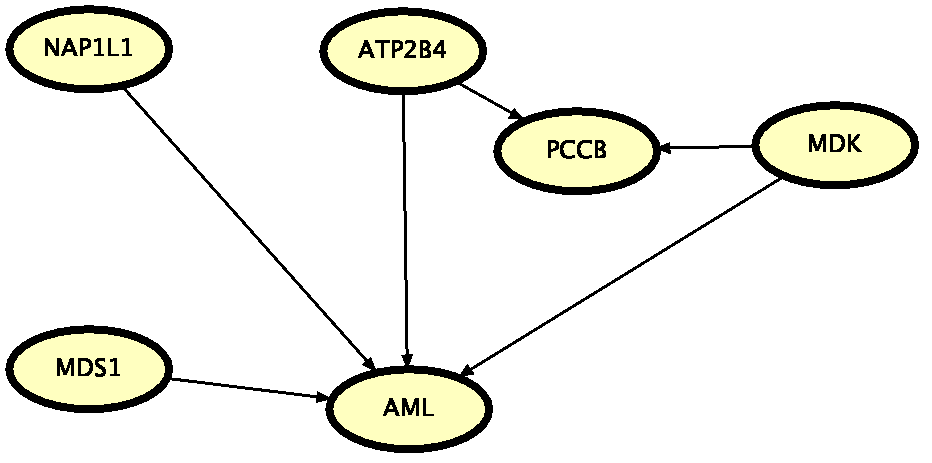
\includegraphics[height=3cm]{images/NPC}
\end{center}
As for the testing, an error rate of $21.43\%$ was obtained while the confusion matrix is shown in the following picture.
\begin{center}
	\begin{minipage}{\linewidth}
		\begin{minipage}{0.44\linewidth}
			\begin{center}
				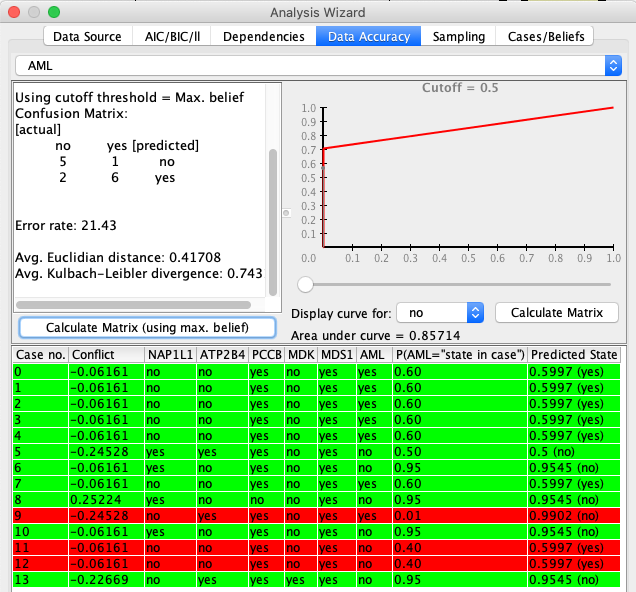
\includegraphics[width=\linewidth]{images/NPCTest}
			\end{center}
		\end{minipage}
		\hspace{0.04\linewidth}
		\begin{minipage}{0.44\linewidth}
			\begin{center}
				\begin{tabular}{c|c|c}
				\diagbox[width=10em]{True}{Pred}&Yes&No\\
				\hline
				Yes								&6	&2\\
				\hline
				No								&1	&5
				\end{tabular}
			\end{center}
		\end{minipage}
	\end{minipage}
\end{center}
From this it's possible to compute scoring values:
\[Acc=\frac{6+5}{6+5+1+2}=\frac{11}{14}=0.78\]
The accuracy is actually $1$ minus the error rate.
\[Prec=\frac{6}{6+1}=0.85\]
\[Rec=\frac{6}{6+2}=0.75\]
\[F_1=\frac{2(0.85+0.75)}{0.85+0.75}=0.8\]
%
%
%
\section*{Greedy Search-and-Score}
\begin{center}
	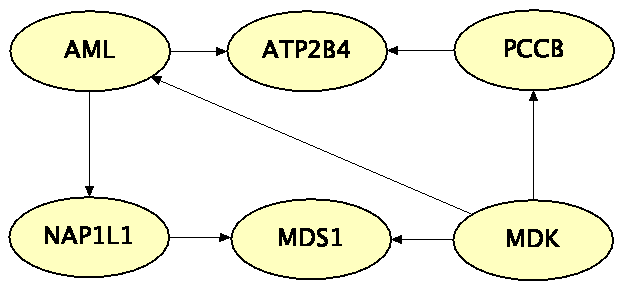
\includegraphics[height=3cm]{images/Greedy}
\end{center}
As for the testing, an error rate of $21.43\%$ was obtained while the confusion matrix is shown in the following picture.
\begin{center}
	\begin{minipage}{\linewidth}
		\begin{minipage}{0.44\linewidth}
			\begin{center}
				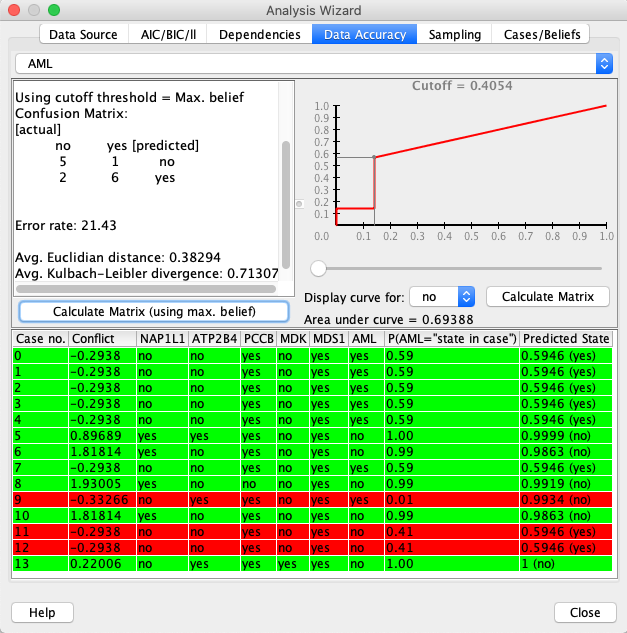
\includegraphics[width=\linewidth]{images/GreedyTest}
			\end{center}
		\end{minipage}
		\hspace{0.04\linewidth}
		\begin{minipage}{0.44\linewidth}
			\begin{center}
				\begin{tabular}{c|c|c}
				\diagbox[width=10em]{True}{Pred}&Yes&No\\
				\hline
				Yes								&6	&2\\
				\hline
				No								&1	&5
				\end{tabular}
			\end{center}
		\end{minipage}
	\end{minipage}
\end{center}
The confusion matrix is the same as before, even though the structure is quite different from before. It's also possible to see that the curve is quite different and the maximum belief is lower, set to 0.4 instead of 0.5. This could be due to the fact that the MDK gene controls greatly the result of AML: indeed, if MDK is set as evidence in Hugin, the probability of obtaining \texttt{no} in AML is $99.65\%$
\[Acc=\frac{6+5}{6+5+1+2}=\frac{11}{14}=0.78\qquad Prec=\frac{6}{6+1}=0.85\]
\[Rec=\frac{6}{6+2}=0.75\qquad F_1=\frac{2(0.85+0.75)}{0.85+0.75}=0.8\]
%
%
%

\section*{Fixed Naive Bayes}
\begin{center}
	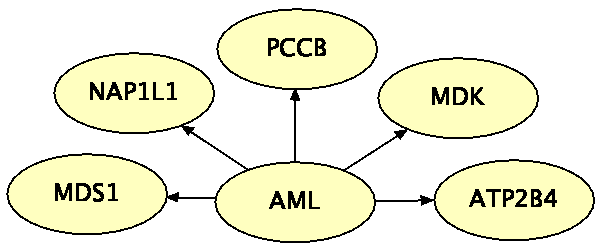
\includegraphics[height=3cm]{images/FixedNaiveBayes}
\end{center}
As for the testing, an error rate of $21.43\%$ was obtained while the confusion matrix is shown in the following picture.
\begin{center}
	\begin{minipage}{\linewidth}
		\begin{minipage}{0.44\linewidth}
			\begin{center}
				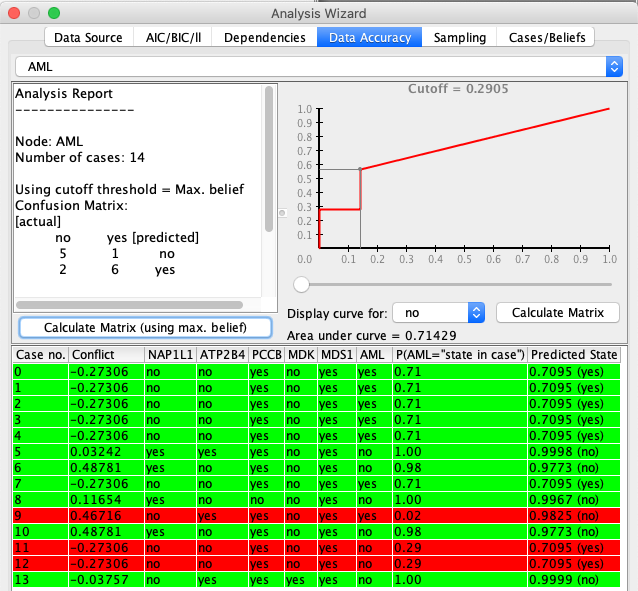
\includegraphics[width=\linewidth]{images/FixedNaiveBayesTest}
			\end{center}
		\end{minipage}
		\hspace{0.04\linewidth}
		\begin{minipage}{0.44\linewidth}
			\begin{center}
				\begin{tabular}{c|c|c}
				\diagbox[width=10em]{True}{Pred}&Yes&No\\
				\hline
				Yes								&6	&2\\
				\hline
				No								&1	&5
				\end{tabular}
			\end{center}
		\end{minipage}
	\end{minipage}
\end{center}
The confusion matrix is the same as the two previous examples, even though the structure is different again.
\[Acc=\frac{6+5}{6+5+1+2}=\frac{11}{14}=0.78\qquad Prec=\frac{6}{6+1}=0.85\]
\[Rec=\frac{6}{6+2}=0.75\qquad F_1=\frac{2(0.85+0.75)}{0.85+0.75}=0.8\]
%
%
%
\section*{Conclusions}
All the three learning algorithms return similar results. This could be due to a gene controlling the AML result more strictly or to the fact that actually the dataset is too small to show differences in the learning algorithm.






	\endgroup
	
\end{document}
